\tikzstyle{op} = [draw, rectangle, anchor=north west,
                  minimum height=1cm, inner sep=0mm]

\def\cR{red!80!white};
\def\cC{green!80!yellow};
\def\cW{blue!60!cyan!80!gray};

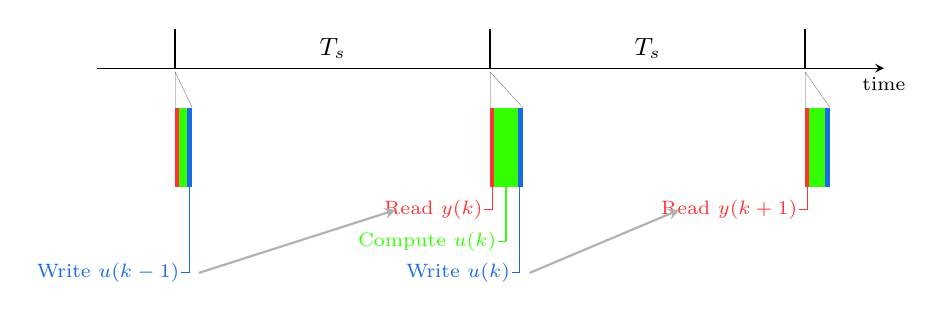
\begin{tikzpicture}[auto,>=stealth]

\draw[->] (0,0)
     -- node[pos=1,below]{\scriptsize{time}}
     (10cm,0);

\node[anchor=south] at (3cm,0mm) {\small{$T_s$}};
\node[anchor=south] at (7cm,0mm) {\small{$T_s$}};

\draw[thick] (1cm,0) -+++(0,5mm);
\node[op,\cR,fill=\cR,minimum width=0.5mm]
     at (1cm,-5mm)
     (R1) {};
\node[op,\cC,fill=\cC,minimum width=1mm]
     at (1.05cm,-5mm)
     (C1) {};
\node[op,\cW,fill=\cW,minimum width=0.5mm]
      at (1.15cm,-5mm)
     (W1) {};
\draw[gray!70!black,ultra thin]
     (R1.north west) --++ (0,4.5mm) -- (W1.north east);

\draw[thick] (5cm,0) -+++(0,5mm);
\node[op,\cR,fill=\cR,minimum width=0.5mm]
     at (5cm,-5mm)
     (R2) {};
\node[op,\cC,fill=\cC,minimum width=3mm]
     at (5.05cm,-5mm)
     (C2) {};
\node[op,\cW,fill=\cW,minimum width=0.5mm]
      at (5.35cm,-5mm)
     (W2) {};
\draw[gray!70!black,ultra thin]
     (R2.north west) --++ (0,4.5mm) -- (W2.north east);

\draw[thick] (9cm,0) -+++(0,5mm);
\node[op,\cR,fill=\cR,minimum width=0.5mm]
     at (9cm,-5mm)
     (R3) {};
\node[op,\cC,fill=\cC,minimum width=2mm]
     at (9.05cm,-5mm)
     (C3) {};
\node[op,\cW,fill=\cW,minimum width=0.5mm]
      at (9.25cm,-5mm)
     (W3) {};
\draw[gray!70!black,ultra thin]
     (R3.north west) --++ (0,4.5mm) -- (W3.north east);

\node[\cW,anchor=east] at (1.175cm,-26mm) (capW1)
     {\scriptsize{Write $u(k-1)$}};
\draw[\cW] (capW1.east) --++(0,1.5cm);
\draw[\cW] (capW1.east) --++(-1mm,0);


\node[\cR,anchor=east] at (5.025cm,-18mm) (capR2)
     {\scriptsize{Read $y(k)$}};
\draw[\cR] (capR2.east) --++(0,1cm);
\draw[\cR] (capR2.east) --++(-1mm,0);

\node[\cC,anchor=east] at (5.2cm,-22mm) (capC2)
     {\scriptsize{Compute $u(k)$}};
\draw[\cC] (capC2.east) --++(0,1cm);
\draw[\cC] (capC2.east) --++(-1mm,0);

\node[\cW,anchor=east] at (5.375cm,-26mm) (capW2)
     {\scriptsize{Write $u(k)$}};
\draw[\cW] (capW2.east) --++(0,1.5cm);
\draw[\cW] (capW2.east) --++(-1mm,0);

\node[\cR,anchor=east] at (9.025cm,-18mm) (capR3)
     {\scriptsize{Read $y(k+1)$}};
\draw[\cR] (capR3.east) --++(0,1cm);
\draw[\cR] (capR3.east) --++(-1mm,0);

\draw[->,thick,gray!60!white]
     (1.3cm,-26mm) --++(25mm,8mm);
\draw[->,thick,gray!60!white]
     (5.5cm,-26mm) --++(19mm,8mm);

\end{tikzpicture}
